%!TEX root =../../course-notes.tex
% ^ leave for LaTeXTools build functionality

\newcommand{\systemWithOneSolutionA}{
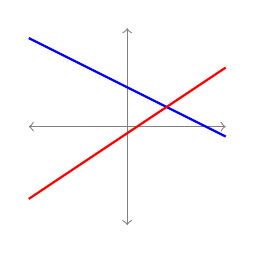
\begin{tikzpicture}[scale=0.25]
\draw[thin,gray,<->] (-5,0) -- (5,0);
\draw[thin,gray,<->] (0,-5) -- (0,5);
\draw[thick,blue] (-5,4.5) -- (5,-0.5);
\draw[thick,red] (-5,-3.67) -- (5,3);
\end{tikzpicture}
}

\newcommand{\systemWithOneSolutionB}{
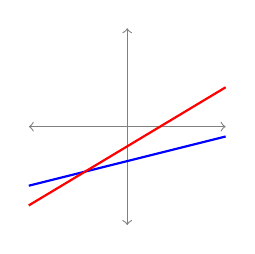
\begin{tikzpicture}[scale=0.25]
\draw[thin,gray,<->] (-5,0) -- (5,0);
\draw[thin,gray,<->] (0,-5) -- (0,5);
\draw[thick,blue] (-5,-3) -- (5,-0.5);
\draw[thick,red] (-5,-4) -- (5,2);
\end{tikzpicture}
}

\newcommand{\systemWithInfinitelyManySolutions}{
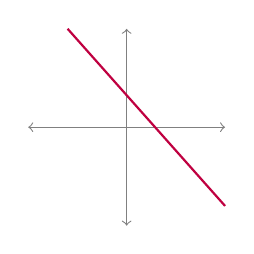
\begin{tikzpicture}[scale=0.25]
\draw[thin,gray,<->] (-5,0) -- (5,0);
\draw[thin,gray,<->] (0,-5) -- (0,5);
\draw[thick,purple] (-3,5) -- (5,-4);
\end{tikzpicture}
}

\newcommand{\systemWithNoSolutions}{
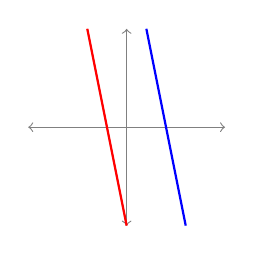
\begin{tikzpicture}[scale=0.25]
\draw[thin,gray,<->] (-5,0) -- (5,0);
\draw[thin,gray,<->] (0,-5) -- (0,5);
\draw[thick,blue] (3,-5) -- (1,5);
\draw[thick,red] (0,-5) -- (-2,5);
\end{tikzpicture}
}
